\chapter[RESULTADOS]{Resultados e Desenvolvimento da Solução}

\section{Análise dos Resultados da Pesquisa}

\subsection{Objetivo da pesquisa}

A pesquisa aplicada com os estudantes da Faculdade do Gama (FCTE) teve como objetivo compreender, de forma exploratória, os hábitos de busca por informações institucionais, as principais dificuldades enfrentadas durante a graduação e o nível de interesse por soluções automatizadas, como chatbots, para apoiar o acesso a esse tipo de conteúdo, os temas mais recorrentes de dúvida ou insegurança acadêmica, de modo a orientar a definição de requisitos e a modelagem dos fluxos de atendimento da aplicação proposta.

\subsubsection{Perfil dos respondentes}

A primeira seção do questionário teve como objetivo caracterizar o perfil dos estudantes participantes da pesquisa. Ao todo, foram obtidas respostas de alunos de quatro dos cinco cursos de graduação ofertados pela Faculdade do Gama (FCTE) da Universidade de Brasília (UnB). A maior parte dos respondentes (75\%) pertence ao curso de Engenharia de Software, seguido por 12{,}5\% de Engenharia Aeroespacial, 6{,}3\% de Engenharia de Energia e 6{,}3\% de Engenharia Automotiva. Nenhum estudante do curso de Engenharia Eletrônica respondeu ao formulário, o que indica uma ausência de representação desse grupo na amostra coletada.

Com relação ao período atual no curso, os respondentes apresentaram uma distribuição ampla, com predominância nos períodos iniciais e finais da graduação. Foram registradas respostas de alunos do 3º, 4º, 5º, 6º, 7º, 10º e 11º períodos, sendo o 3º e o 7º os mais frequentes. Esse recorte é relevante, pois representa tanto estudantes que estão ingressando na vida acadêmica quanto aqueles que estão em fase avançada de integralização curricular, oferecendo perspectivas diversas quanto às dificuldades enfrentadas ao longo do curso.

Além disso, todos os participantes declararam estar matriculados como alunos regulares da UnB, não havendo registros de estudantes em mobilidade acadêmica ou com matrícula especial. Isso reforça o alinhamento entre o público-alvo da pesquisa e os objetivos do projeto, que visa oferecer uma ferramenta de apoio a demandas institucionais recorrentes entre alunos da própria unidade.

\subsubsection{Acesso e dificuldades no uso de informações institucionais}

A segunda seção do questionário teve como propósito investigar os hábitos dos estudantes da FCTE quanto à busca por informações institucionais, bem como mapear as principais dificuldades encontradas nesse processo.

Com relação à frequência com que os alunos buscam esse tipo de informação, os dados indicam que a maior parte dos respondentes (62{,}5\%) realiza essa busca de forma ocasional. Outros 31{,}3\% afirmaram fazê-lo com frequência, enquanto apenas 6{,}3\% relataram buscar informações raramente. Esse resultado demonstra que a consulta a normas, procedimentos e regras da universidade faz parte da rotina da maioria dos estudantes, embora nem sempre de forma contínua.

Sobre os canais mais utilizados para essa busca, os participantes puderam selecionar múltiplas opções. A maioria relatou recorrer a colegas ou veteranos (n = 15), seguido do site da UnB (n = 11) e das redes sociais ou fóruns não oficiais (n = 7). Além disso, seis estudantes indicaram a coordenação do curso como fonte, e outros seis citaram regulamentos ou documentos oficiais. Apenas um respondente relatou o uso de inteligência artificial. Esses dados revelam uma tendência ao uso de fontes informais e interpessoais como principais formas de obter informação, o que pode indicar tanto praticidade quanto carência de sistemas institucionais acessíveis e centralizados.

Questionados sobre a dificuldade em localizar informações oficiais da universidade, 50\% dos estudantes afirmaram que sim, sentem dificuldade, enquanto 43{,}8\% disseram que às vezes enfrentam esse problema. Apenas 6{,}3\% dos respondentes indicaram não ter dificuldades. Para aprofundar essa questão, os participantes que responderam “sim” ou “às vezes” foram convidados a indicar qual é a principal dificuldade enfrentada. A resposta mais frequente foi a falta de orientação sobre onde procurar (56{,}3\%), seguida da dispersão das informações em múltiplos locais (31{,}3\%) e da presença de documentos desatualizados ou confusos (12{,}5\%). Nenhum aluno apontou a linguagem técnica como principal barreira.

Esses resultados reforçam a relevância do problema proposto neste trabalho. A descentralização da informação, aliada à falta de orientação institucional clara, contribui significativamente para o cenário de desinformação percebido pelos alunos. Esse contexto justifica a adoção de uma ferramenta automatizada e centralizadora, como um chatbot, para facilitar o acesso às informações acadêmicas e administrativas mais demandadas.

\subsubsection{Dúvidas acadêmicas e barreiras procedimentais}

Esta seção do questionário teve como foco identificar quais temas acadêmicos costumam gerar maior insegurança entre os estudantes da FCTE, além de investigar se a falta de compreensão dos procedimentos institucionais já resultou em prejuízos concretos, como a não realização de atividades obrigatórias ou oportunidades perdidas.

Os resultados apontam que os assuntos que mais causam dúvida ou insegurança durante a trajetória acadêmica dos alunos estão relacionados, sobretudo, a estágios (n = 15), atividades complementares e de extensão (n = 13), e aproveitamento de disciplinas cursadas em outras instituições (n = 10). Outros tópicos que também apresentaram alta recorrência foram trancamento de matrícula (n = 9), mudança de curso (n = 9), IRA e Média Ponderada (n = 9), dupla diplomação (n = 9), dúvidas sobre o sistema SIGAA (n = 9), e o próprio Projeto Pedagógico de Curso (PPC), igualmente com nove menções. Esses dados demonstram que há uma diversidade de tópicos administrativos e curriculares que geram incertezas, mesmo entre alunos dos períodos mais avançados.

Além disso, mais da metade dos respondentes (56{,}3\%) afirmaram já ter deixado de realizar algum procedimento acadêmico por não entender corretamente seu funcionamento. Entre os procedimentos citados como não realizados devido à falta de clareza estão: aproveitamento de disciplinas (inclusive em língua estrangeira), estágios obrigatórios, bolsas (de tutoria ou auxílio via Cadastro Único), trancamento de matrícula ou do curso e extensão de curso. Tais relatos evidenciam que a falta de orientação acessível pode resultar em atrasos na formação, perda de oportunidades institucionais ou até mesmo impacto negativo no desempenho acadêmico.

A recorrência de dúvidas em torno de processos estruturais da universidade e as consequências práticas relatadas pelos estudantes reforçam a importância da proposta deste trabalho. A centralização e simplificação dessas informações por meio de um chatbot orientado a fluxos institucionais tem potencial para reduzir significativamente essas barreiras.

\subsubsection{Receptividade e expectativas quanto à solução proposta}

A última seção da pesquisa teve como objetivo avaliar a aceitação por parte dos estudantes em relação ao desenvolvimento de um chatbot institucional e identificar suas expectativas quanto às funcionalidades e características dessa ferramenta.

Os resultados demonstraram alta receptividade à proposta: 93{,}8\% dos respondentes afirmaram que utilizariam um chatbot simples para esclarecer dúvidas acadêmicas com base nos regulamentos da FCTE. Apenas 6{,}3\% responderam “talvez”, e nenhum estudante declarou que não utilizaria a ferramenta. Esse resultado indica que há um interesse concreto e imediato por soluções digitais que facilitem o acesso a informações institucionais.

Sobre as funcionalidades esperadas, os participantes indicaram como mais úteis: a resposta a dúvidas frequentes (n = 16), a exibição de prazos e datas importantes (n = 15), e o fornecimento de links diretos para documentos oficiais (n = 12). Também foi sugerida, de forma espontânea, a criação de um manual de instruções que ajude o aluno a compreender como funciona a estrutura acadêmica da faculdade, evidenciando a necessidade de suporte mais amplo para a navegação institucional.

No que diz respeito aos canais preferidos para acesso ao chatbot, as respostas se dividiram entre o Telegram (37{,}5\%) e o site da UnB (37{,}5\%), seguidos pelo WhatsApp (12{,}5\%), site do curso (6{,}3\%) e aplicativo móvel (6{,}3\%). Esse resultado revela que os alunos valorizam soluções acessíveis em plataformas já integradas à sua rotina, como aplicativos de mensagens e canais institucionais oficiais.

Por fim, os participantes também puderam sugerir recursos adicionais que consideram relevantes para inclusão no chatbot. As sugestões envolveram aspectos técnicos e comunicacionais, como: maior dinamismo e fluidez da conversa (com menção a modelos como o GPT), possibilidade de comunicação com professores e secretaria, inclusão de informações sobre auxílios estudantis e a necessidade de uma campanha de divulgação eficaz da ferramenta.

\subsection{Principais \textit{insights} obtidos}

A análise dos dados coletados por meio da pesquisa aplicada com estudantes da Faculdade do Gama (FCTE) permitiu extrair uma série de \textit{insights} relevantes que subsidiam diretamente o desenvolvimento da solução proposta neste trabalho.

Em primeiro lugar, observou-se que o acesso a informações institucionais é uma necessidade frequente entre os estudantes, sendo que mais de 90\% dos participantes relataram buscar esse tipo de conteúdo ao menos ocasionalmente. No entanto, a maior parte dessas buscas é realizada por meio de fontes informais, como colegas, veteranos e redes sociais, o que evidencia a ausência de um canal centralizado, acessível e confiável dentro da instituição.

Outro ponto importante foi a identificação de dificuldades recorrentes no entendimento e cumprimento de procedimentos acadêmicos. Temas como estágios, atividades complementares, trancamento de matrícula, mudanças de curso e aproveitamento de disciplinas foram citados por muitos estudantes como causas de insegurança, além de estarem diretamente associados a relatos de procedimentos que deixaram de ser realizados por falta de compreensão.

Também se constatou que a falta de orientação sobre onde encontrar as informações e a dispersão do conteúdo institucional em múltiplos canais são os principais entraves relatados. A linguagem técnica, por outro lado, não foi apontada como obstáculo, sugerindo que a principal barreira está na estruturação e na forma de disponibilização da informação, e não necessariamente em sua complexidade conceitual.

Por fim, os dados revelaram uma aceitação positiva da proposta de criação de um chatbot institucional. A maioria dos respondentes declarou que utilizaria a ferramenta, destacando como funcionalidades mais desejadas a exibição de dúvidas frequentes, prazos importantes e links diretos para documentos. A preferência por canais de acesso como Telegram, site institucional e WhatsApp reforça a importância de integrar o sistema a plataformas já utilizadas pelos alunos.

Esses resultados confirmam a pertinência da proposta e orientam diretamente o processo de definição de requisitos, modelagem de fluxos e priorização de funcionalidades. A partir dos insights obtidos, torna-se possível projetar um sistema mais alinhado às reais demandas da comunidade acadêmica, contribuindo para a redução das lacunas informacionais atualmente existentes.

\section{Benchmarking de Soluções Existentes}

\subsection{Objetivo do benchmarking}

O \textit{benchmarking} foi adotado neste trabalho como uma estratégia complementar à pesquisa aplicada com os estudantes, com o objetivo de analisar soluções já existentes no domínio de sistemas automatizados de atendimento acadêmico. Essa abordagem busca identificar padrões de funcionamento, funcionalidades recorrentes, boas práticas de interação e aspectos de usabilidade presentes em ferramentas similares, especialmente aquelas implementadas por outras instituições de ensino superior.

Ao observar o funcionamento de ferramentas já aplicadas no contexto educacional, espera-se extrair lições que possam ser adaptadas à realidade da Universidade de Brasília (UnB), promovendo uma solução mais eficaz, contextualizada e alinhada às expectativas dos usuários. Dessa forma, o benchmarking contribui para a minimização de riscos de projeto e para a antecipação de necessidades que, por vezes, não emergem diretamente em etapas exploratórias.

Assim, esta etapa metodológica reforça a proposta centrada no usuário ao incorporar não apenas a perspectiva dos estudantes, mas também o aprendizado obtido a partir de experiências bem-sucedidas em contextos similares.

\subsection{Soluções analisadas e critérios de seleção}

A etapa de benchmarking consistiu na análise de sistemas automatizados de atendimento utilizados por instituições de ensino superior, com foco especial em plataformas que disponibilizam assistentes virtuais ou chatbots para orientação ao público. O objetivo foi identificar funcionalidades, abordagens de interação e possíveis referências para o desenvolvimento do chatbot proposto neste trabalho.

A prospecção contemplou tanto universidades públicas quanto privadas, priorizando aquelas que disponibilizavam canais de atendimento automatizado acessíveis sem a necessidade de autenticação interna. Para isso, foram realizadas buscas diretas nos sites institucionais, bem como simulações de interações com sistemas automatizados encontrados em páginas de contato, áreas de matrículas e FAQs.

Entretanto, observou-se que a maioria dos bots disponíveis ao público está voltada para o atendimento comercial, especialmente em instituições privadas. Esses sistemas apresentam interações padronizadas, geralmente iniciadas por menus fixos com múltiplas opções de seleção, e conduzem o usuário rapidamente a um redirecionamento para atendimento humano, geralmente via WhatsApp, com o objetivo de concluir um processo de venda ou inscrição.

Apesar das limitações de acesso aos sistemas acadêmicos internos, muitas vezes restritos por login institucional, foi possível observar alguns padrões relevantes, como a utilização de menus com múltipla seleção, linguagem objetiva e progressão por etapas curtas. Portanto, ainda que os sistemas acessados não tenham sido voltados diretamente para atendimento acadêmico contínuo, tais aspectos foram considerados como boas práticas e influenciaram decisões de usabilidade na proposta aqui desenvolvida.

\subsection{Resumo do benchmarking realizado}

Durante o processo de benchmarking, foram analisadas soluções de atendimento automatizado de cinco instituições de ensino superior, com o intuito de identificar boas práticas de usabilidade, padrões de interação e possibilidades de estrutura funcional que pudessem inspirar o desenvolvimento do chatbot proposto. A Tabela~\ref{tab:benchmarking} sintetiza as observações realizadas.

\begin{table}[htbp]
\centering
\caption{Resumo do benchmarking de chatbots em instituições de ensino}
\label{tab:benchmarking}
\begin{tabular}{|p{3.5cm}|p{4.2cm}|p{5.8cm}|}
\hline
\textbf{Instituição} & \textbf{Finalidade do Bot} & \textbf{Aspectos Observados} \\ \hline
Universidade Católica de Brasília & Atendimento comercial & Menu inicial com múltiplas opções; respostas automáticas padronizadas; redirecionamento rápido para WhatsApp. \\ \hline
UniCEUB & Atendimento comercial & Fluxo simples; ausência de FAQ acadêmico; forte foco na captação de alunos e conclusão de matrícula via humano. \\ \hline
Cruzeiro do Sul & Atendimento geral e comercial & Apresentação visual amigável; utilização de menus interativos; linguagem acessível; ausência de integração com sistema acadêmico. \\ \hline
Estácio & Suporte comercial & Múltipla seleção funcional; chatbot como triagem para atendimento humano; direcionamento por áreas de interesse. \\ \hline
Faculdade Única & Atendimento comercial & Opções de navegação objetiva; foco em cursos, inscrições e mensalidades; pouca flexibilidade de diálogo. \\ \hline
\end{tabular}
\end{table}

\subsection{Aprendizados e funcionalidades inspiradas no benchmarking}

Um primeiro aprendizado relevante foi a adoção de \textbf{menus interativos com múltipla seleção}, recurso presente em instituições como a Estácio e a Cruzeiro do Sul. Essa funcionalidade demonstrou-se eficaz na organização das opções de atendimento e na condução do usuário ao conteúdo desejado com maior autonomia.

Outro ponto observado foi a importância de manter uma \textbf{linguagem acessível e objetiva}, com mensagens curtas e claras, que orientem o usuário sem gerar confusão. A utilização de fluxos bem definidos e visualmente amigáveis contribui para reduzir o tempo de resposta e aumentar a sensação de controle na interação.

Apesar do viés comercial predominante nos bots analisados, uma prática comum foi a \textbf{utilização do chatbot como filtro inicial} funcionando como triagem para posterior encaminhamento ao atendimento humano via WhatsApp. Essa abordagem foi inspiradora para o presente projeto, que também adota o modelo de \textbf{atendimento em múltiplos níveis}, permitindo que dúvidas mais complexas sejam encaminhadas à coordenação ou secretaria do curso, caracterizando um atendimento de \textit{nível 2}, conforme discutido na metodologia.

Por fim, a análise evidenciou a carência, nas instituições estudadas, de soluções voltadas ao suporte acadêmico automatizado, o que reforça a \textbf{originalidade e relevância da proposta} do chatbot desenvolvido neste trabalho. O foco na prestação de informações acadêmicas confiáveis, com base em regulamentos oficiais, representa um diferencial frente às soluções existentes, que em geral se limitam a captar novos alunos ou esclarecer dúvidas administrativas simples.

\section{Definição de Requisitos}

\subsection{Metodologia para levantamento de requisitos}

A elicitação de requisitos deste projeto foi conduzida com base em uma abordagem empática e centrada no usuário, alinhada às fases iniciais do Design Thinking, especialmente nas etapas de \textit{imersão} e \textit{definição} \cite{brown2009change}. A aplicação dessa abordagem permitiu a compreensão mais profunda das necessidades reais dos estudantes da Universidade de Brasília do campus Gama (FCTE), contribuindo para a formulação de requisitos que de fato atendam ao contexto e às dificuldades enfrentadas pela comunidade acadêmica.

A primeira técnica utilizada foi a aplicação de uma pesquisa exploratória junto a discentes da Faculdade de Ciência e Tecnologia (FCTE). O questionário estruturado coletou dados tanto quantitativos quanto qualitativos, permitindo levantar percepções sobre a dificuldade de acesso a informações acadêmicas, os canais utilizados para esse fim, as temáticas que mais geram insegurança ao longo da graduação e a receptividade em relação ao uso de um chatbot institucional. Essa investigação empírica foi essencial para identificar padrões de comportamento, expectativas e problemas recorrentes, funcionando como base primária para a definição dos requisitos do sistema.

Em paralelo, foi realizada uma análise de benchmarking com foco em chatbots educacionais de instituições de ensino superior, tanto públicas quanto privadas. Ainda que o acesso aos sistemas internos dessas universidades tenha sido limitado, foi possível identificar boas práticas e funcionalidades recorrentes nos bots de atendimento ao público externo, como a possibilidade de múltiplas seleções de respostas e o redirecionamento automatizado para canais humanos. A comparação com soluções existentes permitiu identificar lacunas e oportunidades para o desenvolvimento do chatbot proposto.

Ambas as técnicas foram utilizadas de forma complementar, uma vez que o benchmarking forneceu insumos de mercado e inspirações funcionais, enquanto a pesquisa com os estudantes permitiu compreender a realidade local e construir soluções sob medida. Essa combinação de abordagens encontra respaldo na literatura de Engenharia de Software, que recomenda a utilização de múltiplas fontes de elicitação para aumentar a acurácia e a utilidade dos requisitos \cite{pressman2016engenharia}.

Assim, o processo de levantamento de requisitos foi conduzido de forma iterativa, empática e fundamentada, alinhado às melhores práticas da Engenharia de Software moderna e às diretrizes metodológicas do Design Thinking.

\subsection{Requisitos funcionais do sistema}

Com base na metodologia adotada para a elicitação de requisitos, fundamentada nas etapas iniciais do Design Thinking, na aplicação de pesquisa exploratória com os estudantes da FCTE e no benchmarking com outras instituições de ensino, foi possível consolidar um conjunto de requisitos funcionais (RF) que nortearão o desenvolvimento do chatbot proposto.

Os requisitos funcionais descrevem as funcionalidades específicas que o sistema deverá ser capaz de realizar, refletindo diretamente as necessidades e expectativas levantadas junto ao público-alvo \cite{pressman2016engenharia}. A Tabela~\ref{tab:requisitos_funcionais} apresenta esses requisitos numerados e descritos de forma clara e objetiva.

\begin{table}[H]
\caption{Requisitos funcionais do chatbot acadêmico}
\label{tab:requisitos_funcionais}
\centering
\begin{tabular}{|c|p{12cm}|}
\hline
\textbf{ID} & \textbf{Descrição do Requisito Funcional} \\
\hline
RF01 & O chatbot deve permitir a consulta de dúvidas frequentes relacionadas à vida acadêmica, como trancamentos, estágios, IRA, entre outros tópicos levantados na pesquisa. \\
\hline
RF02 & O sistema deve apresentar prazos e datas importantes extraídos do calendário acadêmico da UnB. \\
\hline
RF03 & O chatbot deve disponibilizar links diretos para regulamentos e documentos oficiais atualizados. \\
\hline
RF04 & O chatbot deve oferecer uma interface acessível via Telegram e WhatsApp, conforme preferência manifestada pelos respondentes. \\
\hline
RF05 & O sistema deve permitir múltiplas seleções de opções de resposta quando necessário, conforme observado no benchmarking. \\
\hline
RF06 & O chatbot deve identificar quando a dúvida do usuário não pode ser resolvida automaticamente e, nesse caso, encaminhá-lo para um canal de atendimento humano (secretaria ou docente), caracterizando um atendimento de nível 2, conforme o modelo ITIL v4. \\
\hline
\end{tabular}
\end{table}

\subsection{Requisitos não funcionais do sistema}

Além das funcionalidades específicas, o sistema chatbot deve atender a um conjunto de requisitos não funcionais (RNF), os quais tratam das qualidades e restrições globais que influenciam a experiência do usuário, o desempenho, a segurança e a manutenibilidade da solução. Esses requisitos garantem que o software não apenas funcione corretamente, mas também o faça de maneira eficaz e satisfatória \cite{pressman2016engenharia}.

A Tabela~\ref{tab:requisitos_nao_funcionais} apresenta os requisitos não funcionais definidos com base nas boas práticas de Engenharia de Software, nos resultados da pesquisa exploratória com os usuários e nos critérios observados durante o benchmarking.

\begin{table}[H]
\caption{Requisitos não funcionais do chatbot acadêmico}
\label{tab:requisitos_nao_funcionais}
\centering
\begin{tabular}{|c|p{12cm}|}
\hline
\textbf{ID} & \textbf{Descrição do Requisito Não Funcional} \\
\hline
RNF01 & \textbf{Usabilidade}: o chatbot deve apresentar linguagem acessível, interface amigável e interação natural, garantindo que estudantes de diferentes níveis de familiaridade tecnológica possam utilizá-lo sem dificuldades. \\
\hline
RNF02 & \textbf{Confiabilidade}: o sistema deve responder com informações corretas e atualizadas, extraídas de fontes oficiais da UnB, como o Projeto Pedagógico de Curso (PPC), regulamentos e editais. \\
\hline
RNF03 & \textbf{Disponibilidade}: o chatbot deve estar disponível para uso 24 horas por dia, 7 dias por semana, uma vez que a busca por informações pode ocorrer fora do horário administrativo. \\
\hline
RNF04 & \textbf{Desempenho}: o tempo de resposta do chatbot deve ser inferior a 2 segundos, garantindo agilidade no atendimento e evitando frustração do usuário. \\
\hline
RNF05 & \textbf{Portabilidade}: o sistema deve funcionar corretamente nas plataformas Telegram e WhatsApp, conforme a preferência majoritária dos usuários identificada na pesquisa. \\
\hline
RNF06 & \textbf{Manutenibilidade}: o sistema deve ser projetado de forma modular e documentada, facilitando a atualização de informações e a adição de novas funcionalidades futuras. \\
\hline
RNF07 & \textbf{Segurança}: o chatbot não deve solicitar nem armazenar dados sensíveis dos usuários, respeitando os princípios da Lei Geral de Proteção de Dados Pessoais (LGPD) – Lei nº 13.709/2018. \\
\hline
\end{tabular}
\end{table}

\subsection{Priorização de requisitos}
Haja vista a quantidade de funcionalidades elencadas através do levantamento de requisitos e do brainstorming, será utilizada a técnica de priorização de requisitos MoSCoW, que é uma abordagem eficaz para classificação com base na importância de cada exigência \cite{cottrell1999}. Ela se divide em 4 categorias:

        \begin{itemize}
            \item \textbf{\textit{Must Have}}: (Precisa
            ter), são essenciais para o sucesso do projeto
            \item \textbf{\textit{Should Have}}: (Deve ter), são requisitos desejáveis para o sistema, apesar de ser possível a existência do projeto sem eles, mesmo que temporariamente.
            \item \textbf{\textit{Could Have}}: (Pode ter), funcionalidades adicionais que podem ser priorizadas, caso haja tempo.
            \item \textbf{\textit{Won’t Have}}: (não terá agora), requisitos que não terão prioridade durante o desenvolvimento do projeto.
        \end{itemize}

Assim, a priorizacao pode ser conferida na Tabela ~\cite{priorizacao_requisitos}

\begin{table}[H]
\caption{Priorização dos requisitos segundo o modelo MoSCoW}
\label{tab:priorizacao_requisitos}
\centering
\begin{tabular}{|p{9cm}|c|}
\hline
\textbf{Requisito} & \textbf{Prioridade} \\
\hline
RF01: Permitir consulta a dúvidas frequentes baseadas em regulamentos & Must Have \\
\hline
RF02: Exibir prazos e datas importantes com base no calendário acadêmico & Must Have \\
\hline
RF03: Gerar links diretos para documentos oficiais da UnB/FCTE & Should Have \\
\hline
RF04: Encaminhar o usuário para a secretaria ou professor responsável, quando necessário & Must Have \\
\hline
RF05: Armazenar histórico da conversa para fins de melhoria do sistema & Could Have \\
\hline
RNF01: Usabilidade (linguagem acessível e interação amigável) & Must Have \\
\hline
RNF02: Confiabilidade das informações (origem oficial) & Must Have \\
\hline
RNF03: Disponibilidade 24/7 & Should Have \\
\hline
RNF04: Tempo de resposta inferior a 2 segundos & Must Have \\
\hline
RNF05: Portabilidade (funcionar em Telegram e WhatsApp) & Must Have \\
\hline
RNF06: Manutenibilidade (modularidade e documentação) & Should Have \\
\hline
RNF07: Segurança (conformidade com a LGPD) & Must Have \\
\hline
\end{tabular}
\end{table}

\section{Modelagem e Arquitetura da Solução}

Esta seção apresenta a modelagem técnica do sistema proposto, contemplando sua arquitetura geral, os principais componentes envolvidos, as interações entre os módulos e os padrões utilizados no desenvolvimento. A modelagem tem como objetivo estabelecer uma visão clara da estrutura interna do chatbot, evidenciando sua organização, responsabilidades e os fluxos de informação que permitem seu funcionamento.

A definição da arquitetura da solução parte dos requisitos elicitados e das necessidades identificadas ao longo das etapas de pesquisa, com ênfase na simplicidade, escalabilidade e manutenibilidade do sistema. O chatbot foi concebido para operar como uma ferramenta de suporte informacional aos estudantes da Faculdade do Gama da Universidade de Brasília (FCTE/UnB), integrando-se a plataformas populares de mensageria e respondendo a consultas com base em documentos oficiais e regulamentações institucionais.

\subsection{Arquitetura da Solução}

A arquitetura da solução proposta foi concebida com base em princípios de modularidade, escalabilidade e facilidade de integração. A estrutura segue uma abordagem baseada em microsserviços, permitindo a separação clara entre as camadas de interface, lógica de negócios e persistência de dados.

A Figura~\ref{fig:arquitetura} apresenta a arquitetura geral do sistema. O núcleo da aplicação é composto por uma API desenvolvida em \textit{Spring Boot}, responsável por centralizar a lógica de negócios do chatbot. Essa API é hospedada na nuvem da Amazon Web Services (AWS), o que garante maior disponibilidade, escalabilidade e segurança à solução.

Na camada de dados, é utilizado um banco de dados relacional PostgreSQL, que armazena as informações necessárias para o funcionamento do sistema, como diálogos, regras de atendimento, histórico de interações e dados administrativos.

Para a interface com o usuário, a solução oferece um \textit{frontend} desenvolvido em \textit{Next.js}, uma estrutura baseada em React, que proporciona uma experiência de aplicação de página única (SPA). Esse frontend é hospedado na plataforma Vercel, especializada no suporte a aplicações \textit{serverless} modernas.

Além do acesso via navegador, a solução também permite que os usuários interajam com o chatbot através de plataformas de mensagens instantâneas, como WhatsApp e Telegram. Essas integrações ocorrem por meio das APIs específicas dessas plataformas, que se comunicam com a API do chatbot para fornecer respostas automáticas em tempo real.

\begin{figure}[htbp]
    \centering
    
\includegraphics[width=0.6\linewidth]{./figuras/arquitetura.eps}
    \caption{Arquitetura}
    \label{fig:arquitetura}
\end{figure}

\subsection{Protótipo de Baixa Fidelidade}

O desenvolvimento de protótipos é uma etapa fundamental no processo de construção de soluções centradas no usuário, pois permite antecipar a estrutura, o funcionamento e a navegabilidade do sistema proposto antes de sua implementação final. Os protótipos de baixa fidelidade são representações simplificadas que visam avaliar a concepção geral da interface e as principais funcionalidades, sem necessidade de detalhamento estético ou de integração com sistemas complexos.

Neste trabalho, optou-se por utilizar capturas de tela (\textit{screenshots}) diretamente do MVP já desenvolvido como forma de prototipação de baixa fidelidade. Essa decisão se deu em função da limitação de tempo disponível para elaboração de protótipos dedicados, além da existência de um produto funcional minimamente viável que já ilustra de forma eficaz os principais fluxos de interação.

Essa abordagem também é consistente com o modelo de desenvolvimento incremental adotado, em que versões preliminares do sistema são utilizadas como base para refinamentos e validações, conforme preconizado por metodologias ágeis como XP e Scrum.

As imagens apresentadas a seguir demonstram as principais telas e interações do chatbot, permitindo uma análise visual e funcional da solução proposta, bem como auxiliando na validação junto aos usuários e stakeholders.

\begin{figure}[h]
	\centering
	
\includegraphics[width=1\linewidth]{./figuras/tela de login.eps}
	\caption{Tela de Login}
	\footnotesize Fonte: Autores.
	\label{fig02}
\end{figure}

\begin{figure}[h]
	\centering
	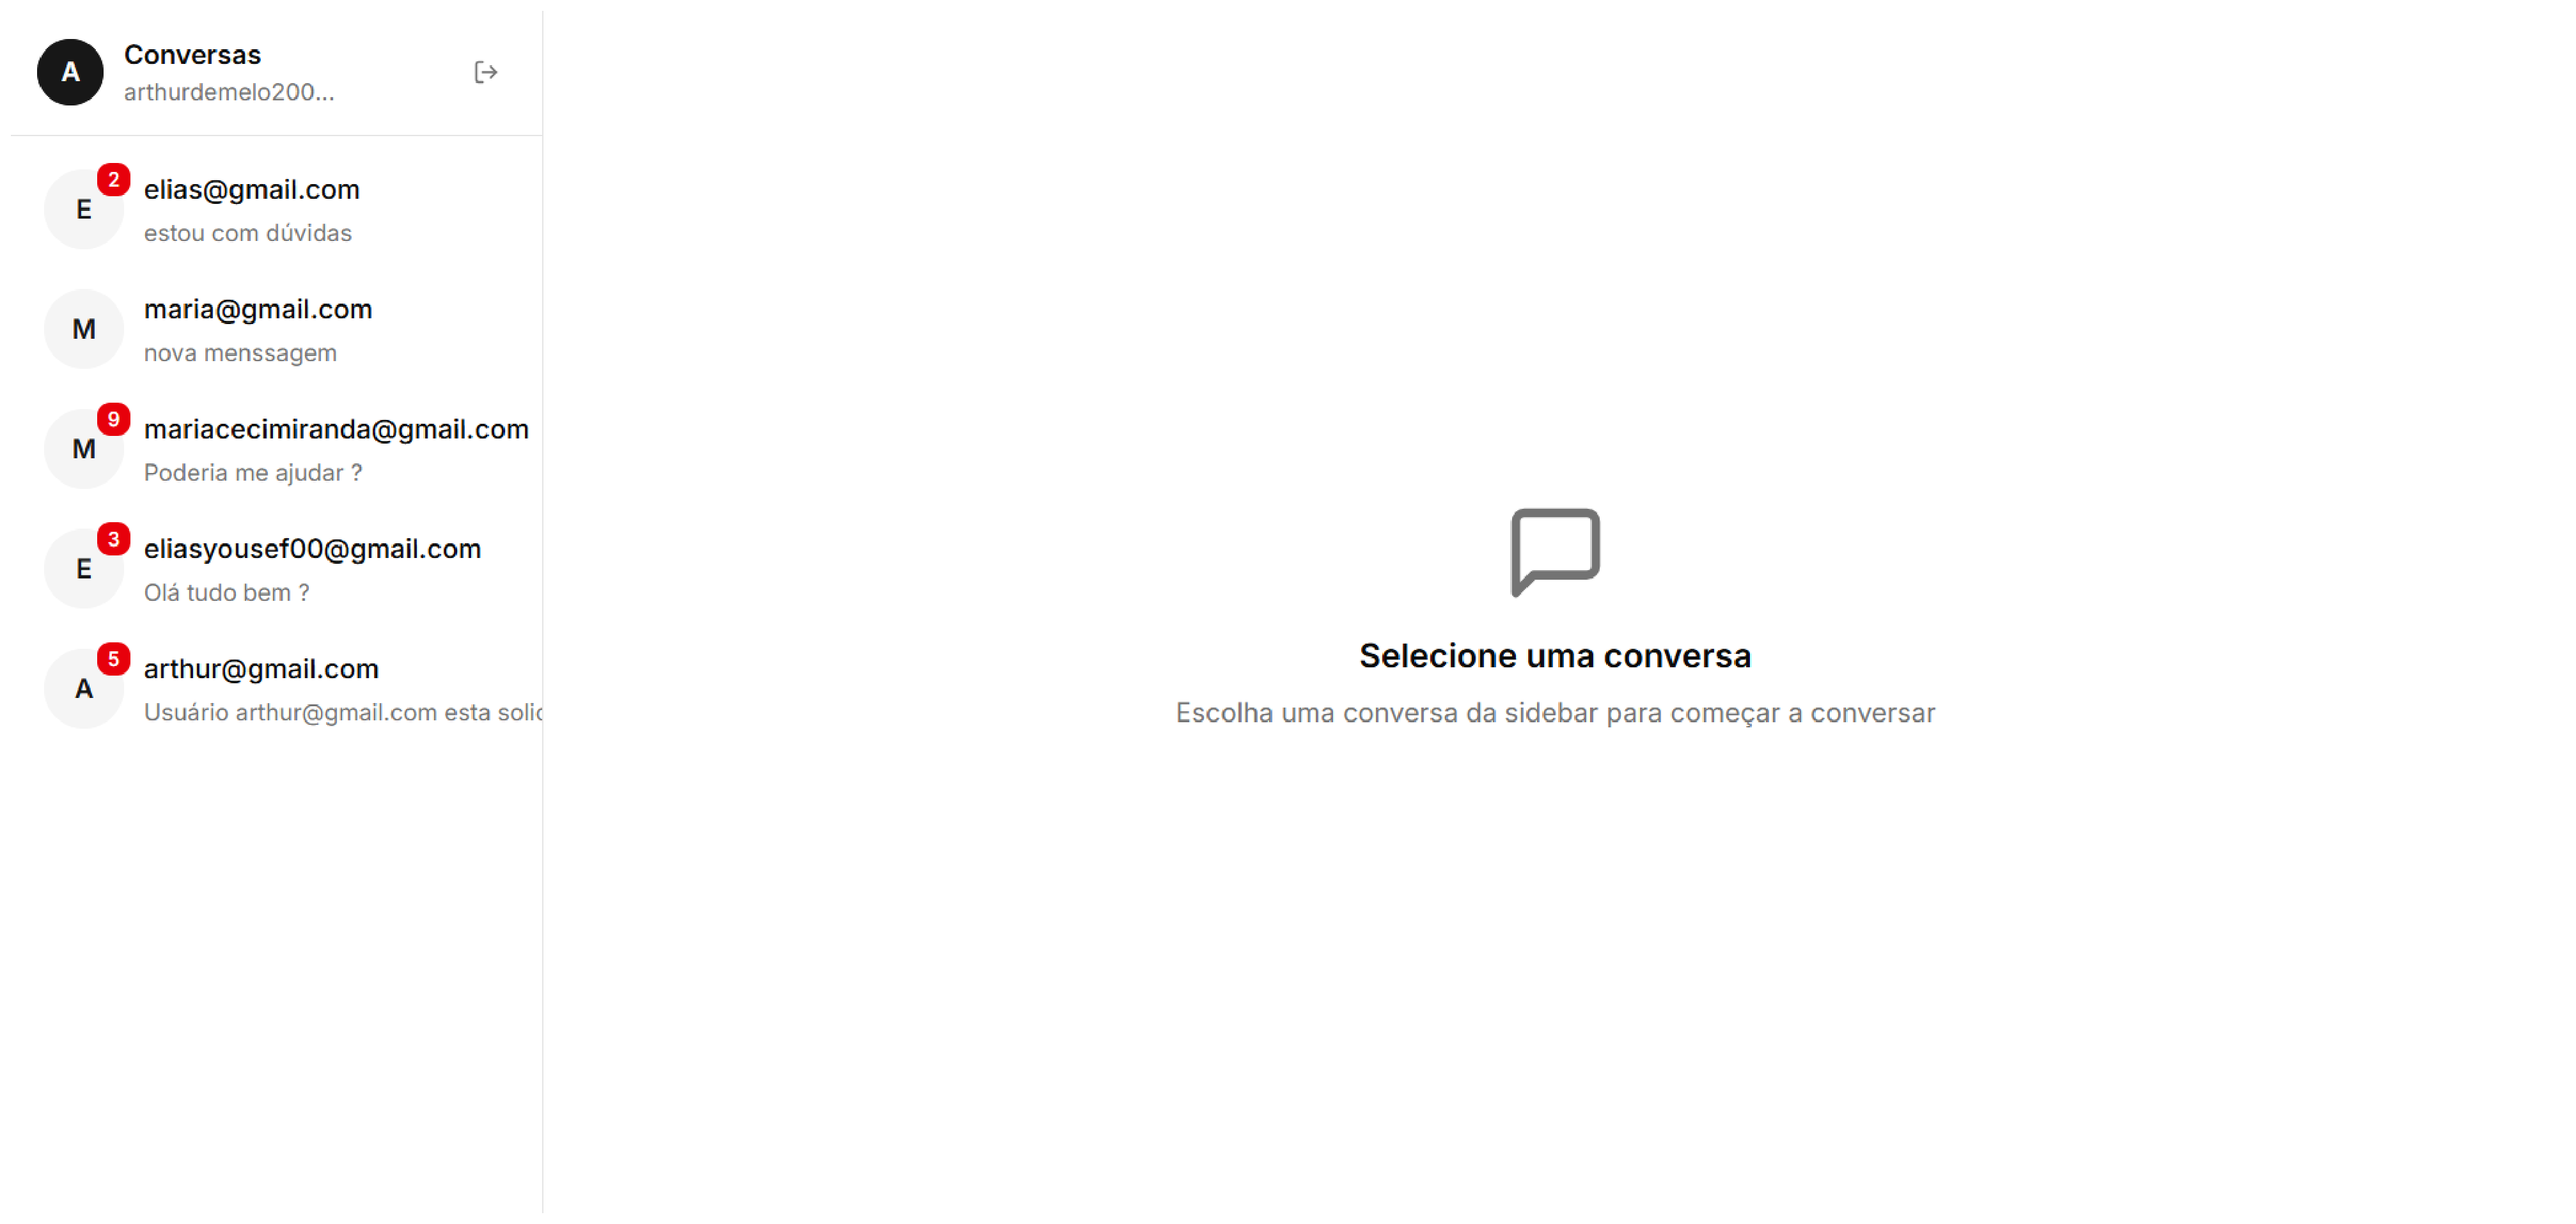
\includegraphics[width=1\linewidth]{./figuras/tela principal.eps}
	\caption{Tela principal}
	\footnotesize Fonte: Autores.
	\label{fig03}
\end{figure}

\begin{figure}[h]
	\centering
	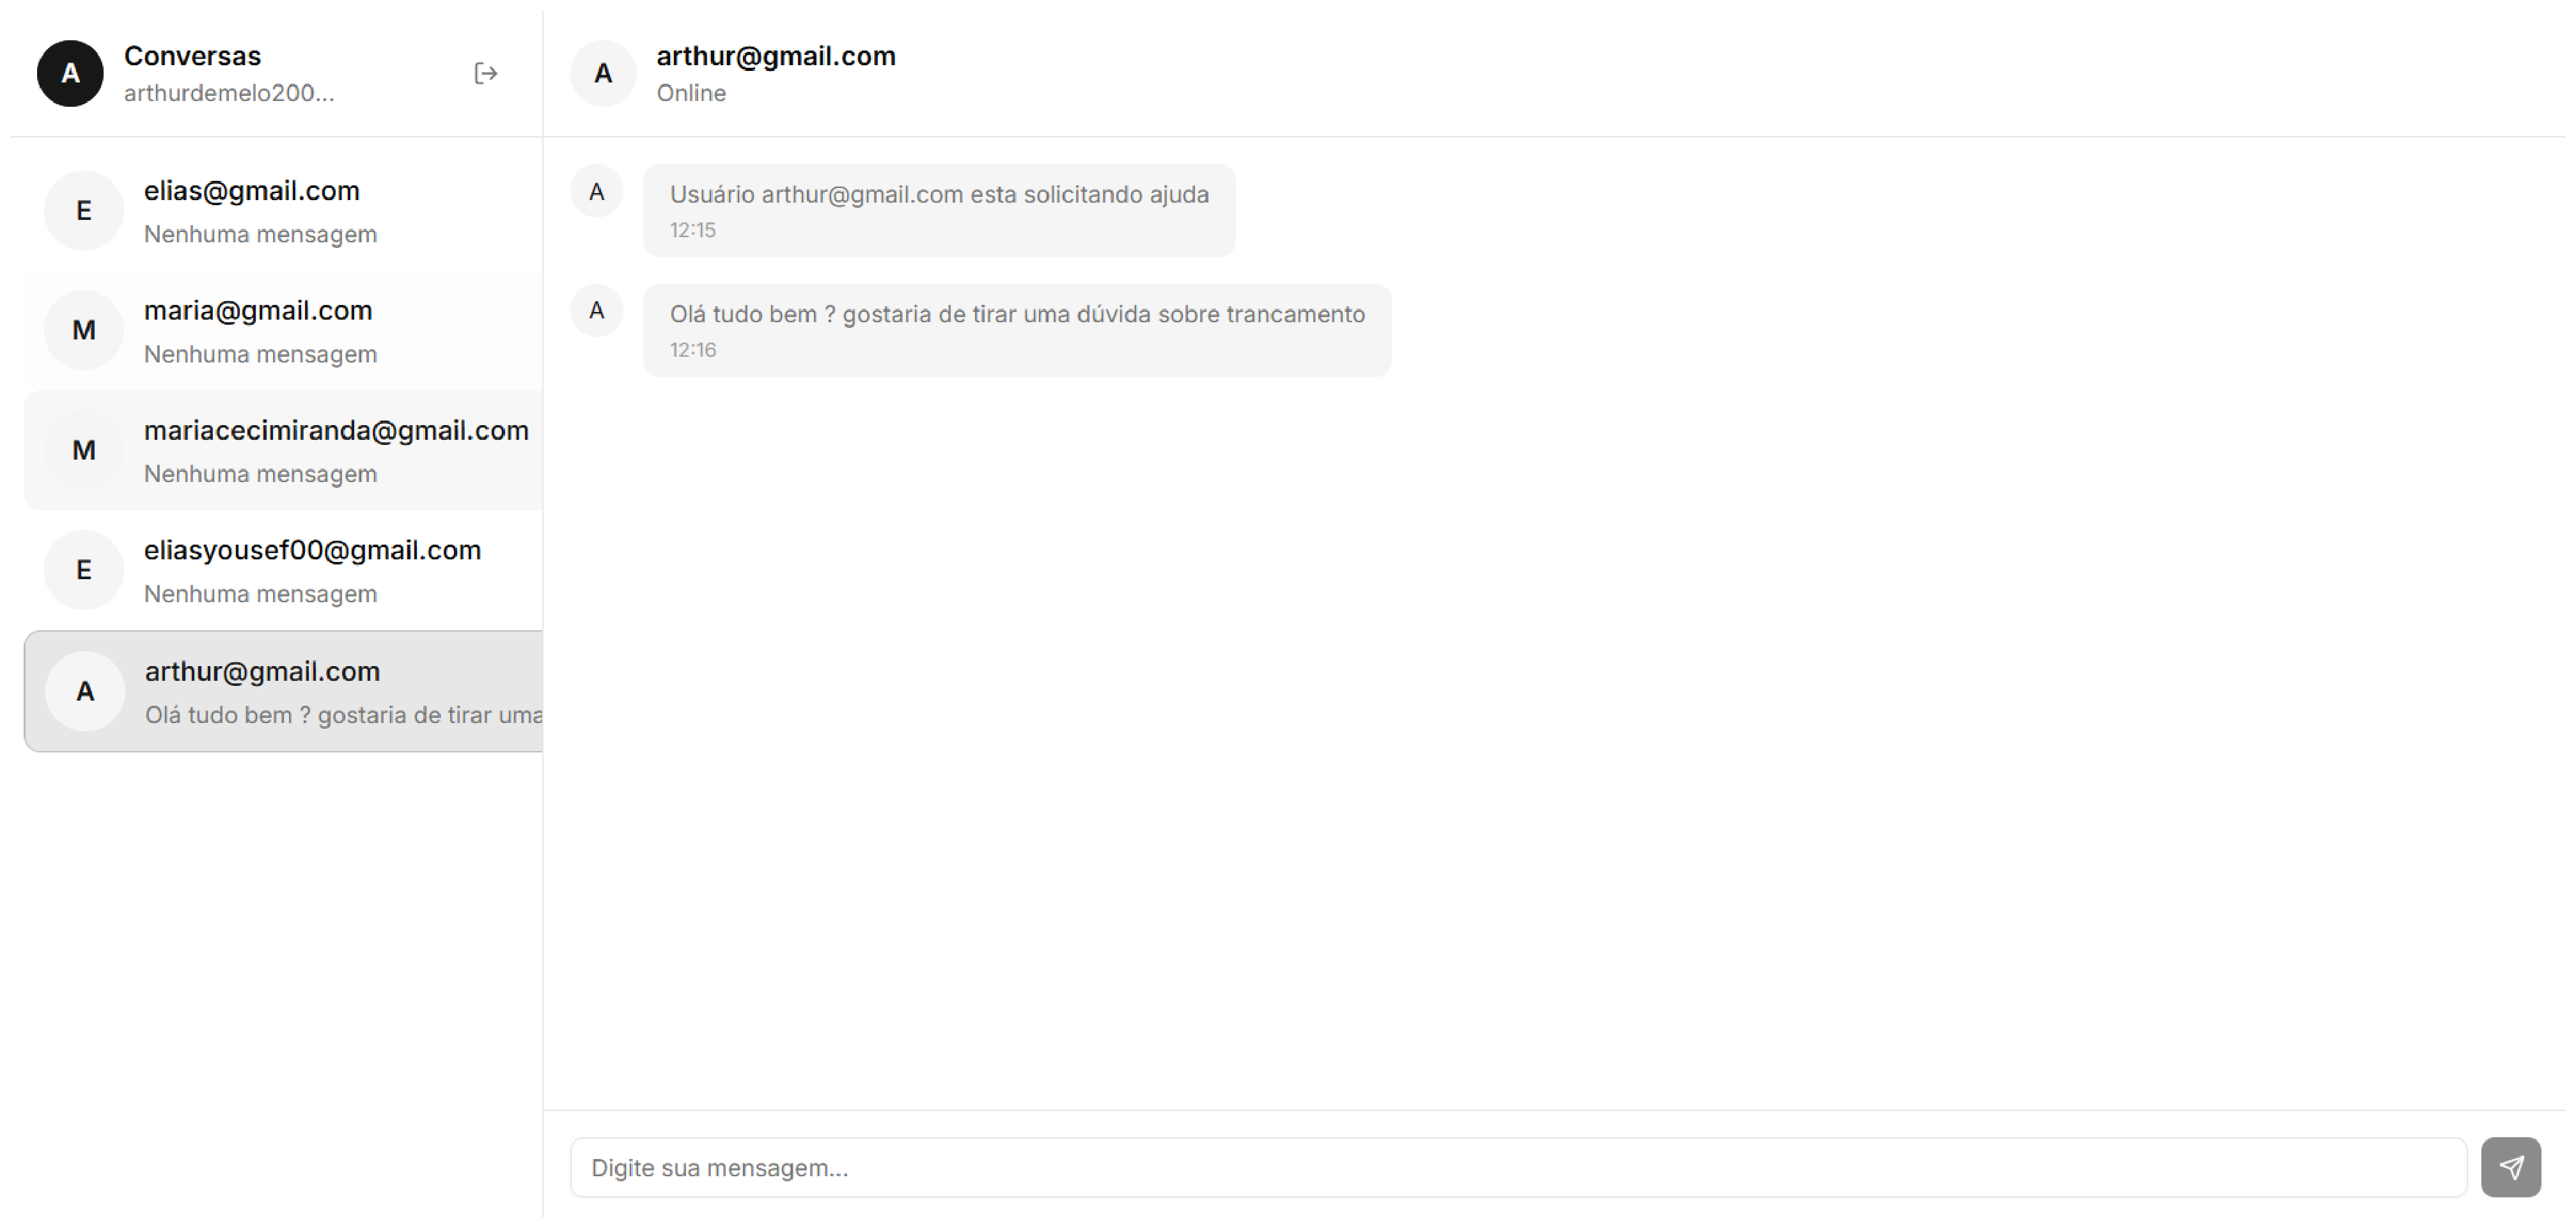
\includegraphics[width=1\linewidth]{./figuras/tela conversa.eps}
	\caption{Tela de conversa}
	\footnotesize Fonte: Autores.
	\label{fig04}
\end{figure}

\begin{figure}[h]
	\centering
	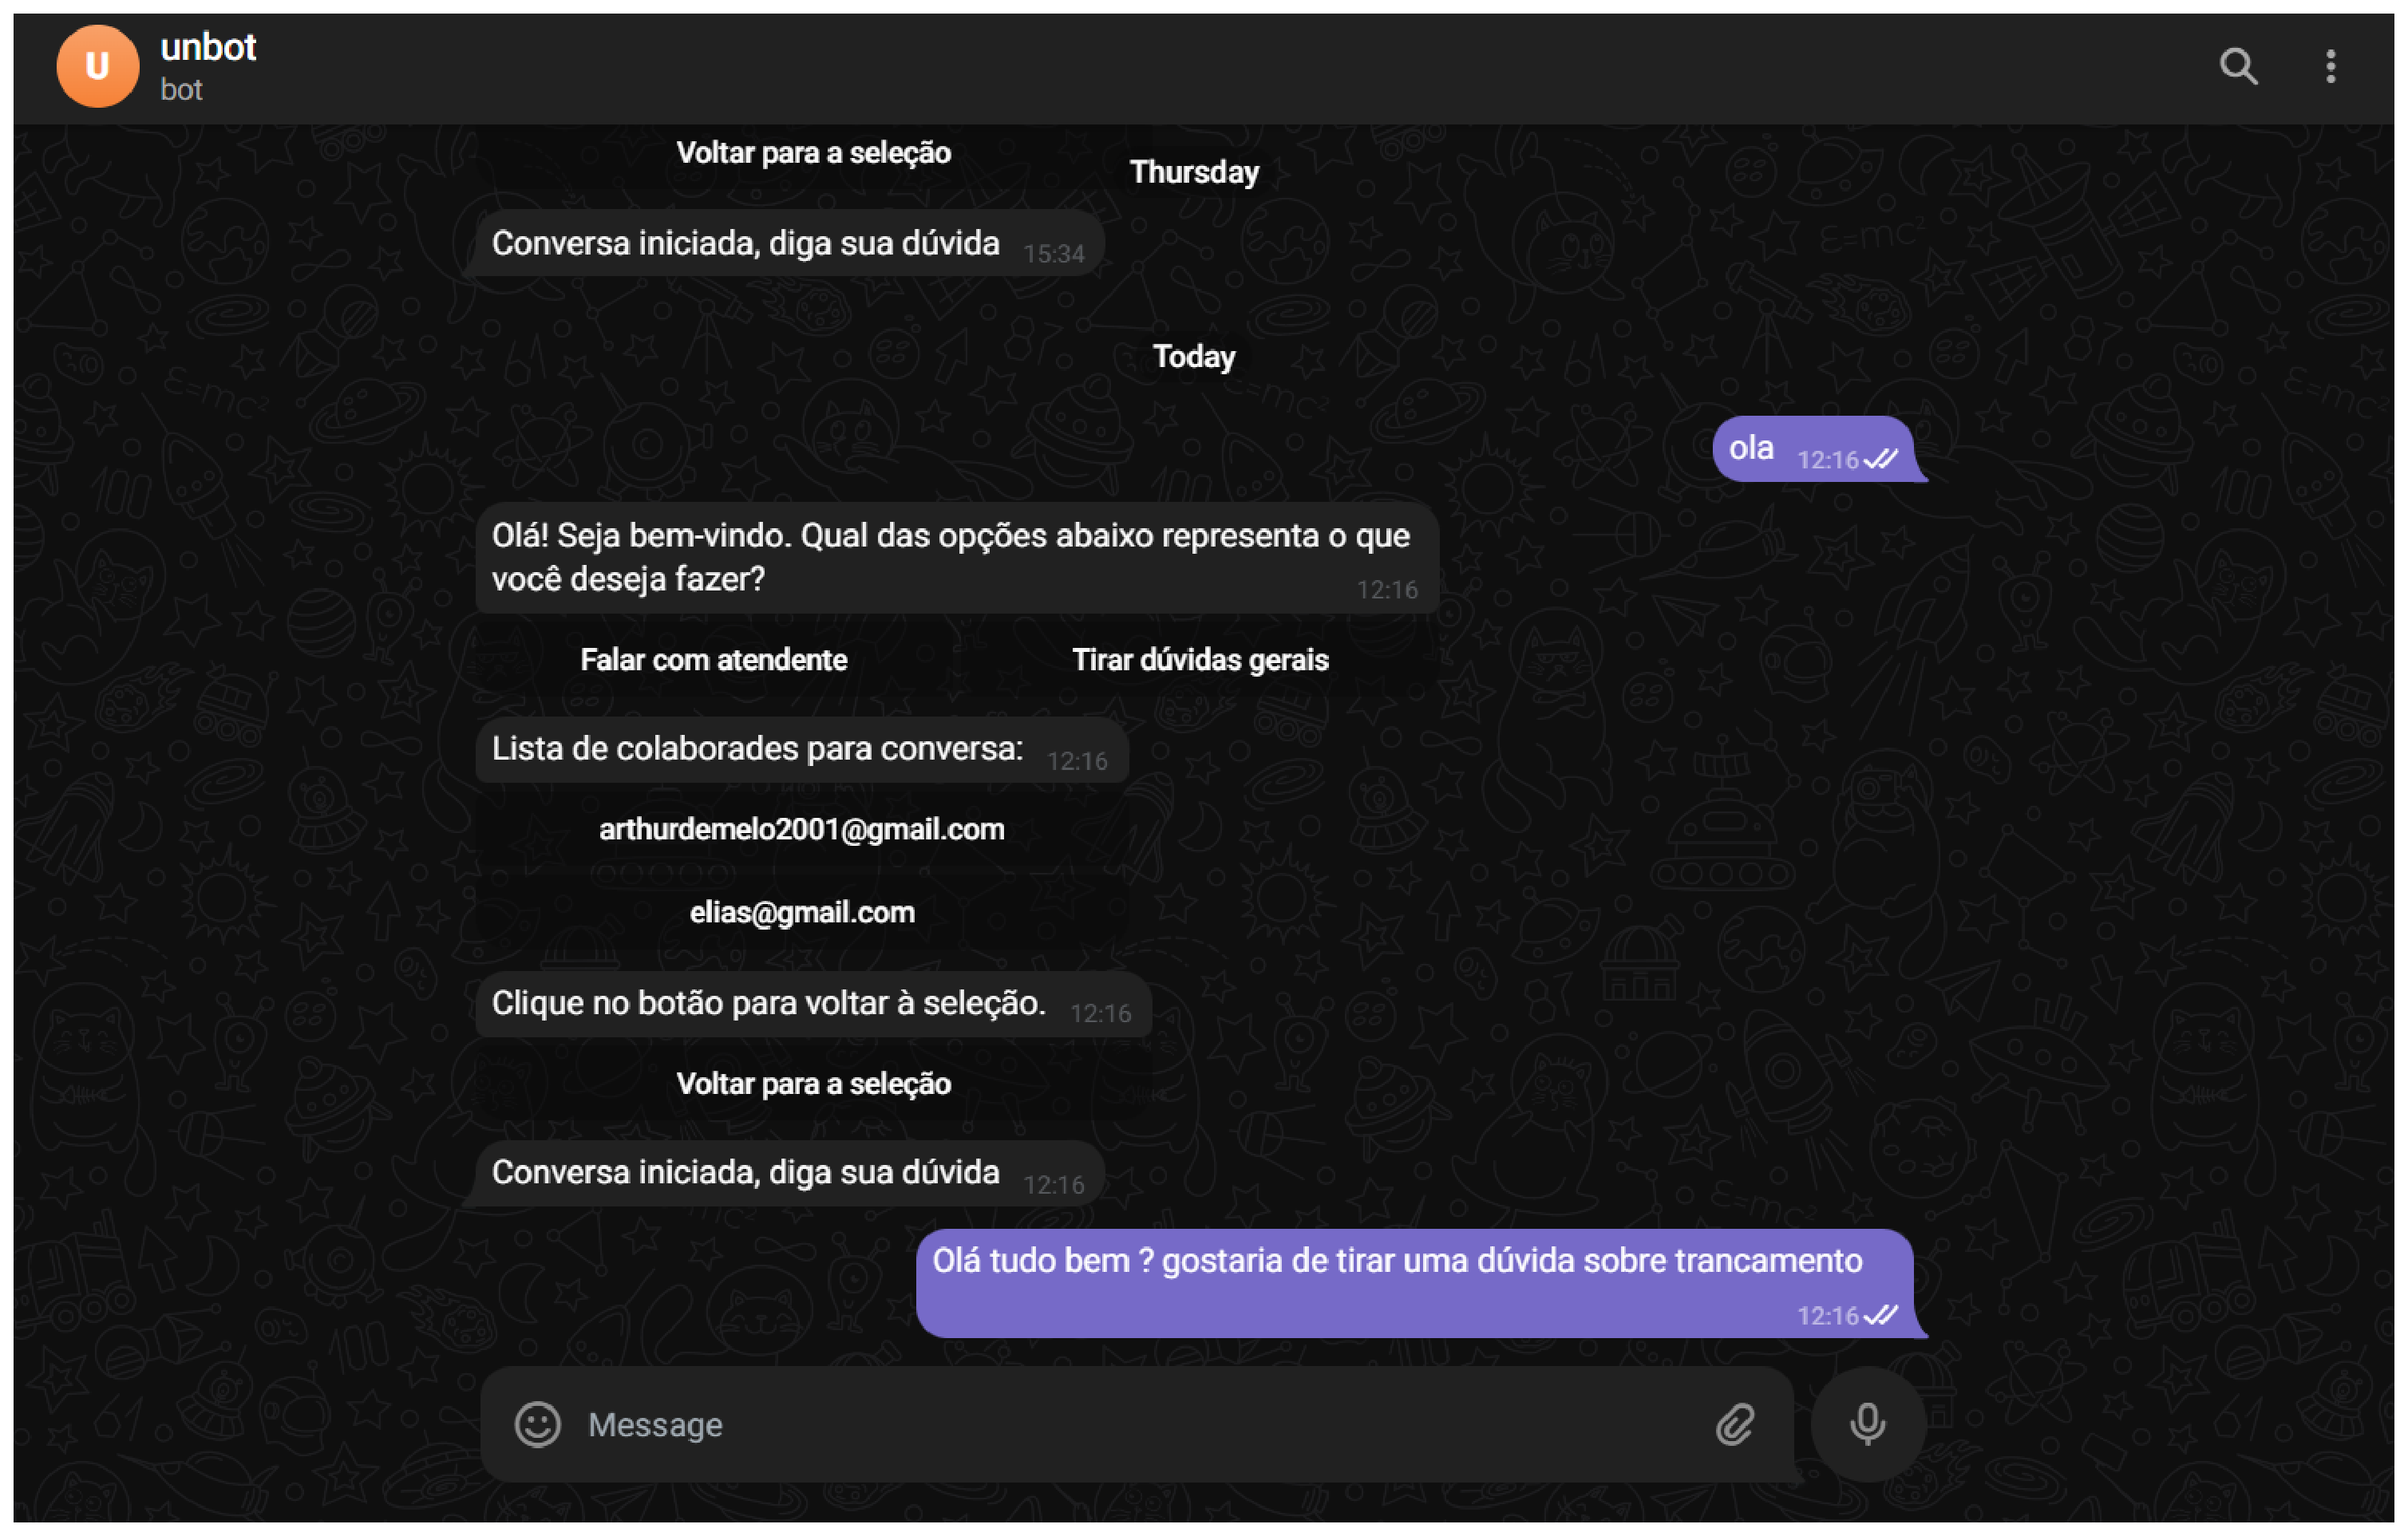
\includegraphics[width=1\linewidth]{./figuras/tela conversa bot.eps}
	\caption{Tela de conversa com o Bot}
	\footnotesize Fonte: Autores.
	\label{fig05}
\end{figure}

\begin{figure}[h]
	\centering
	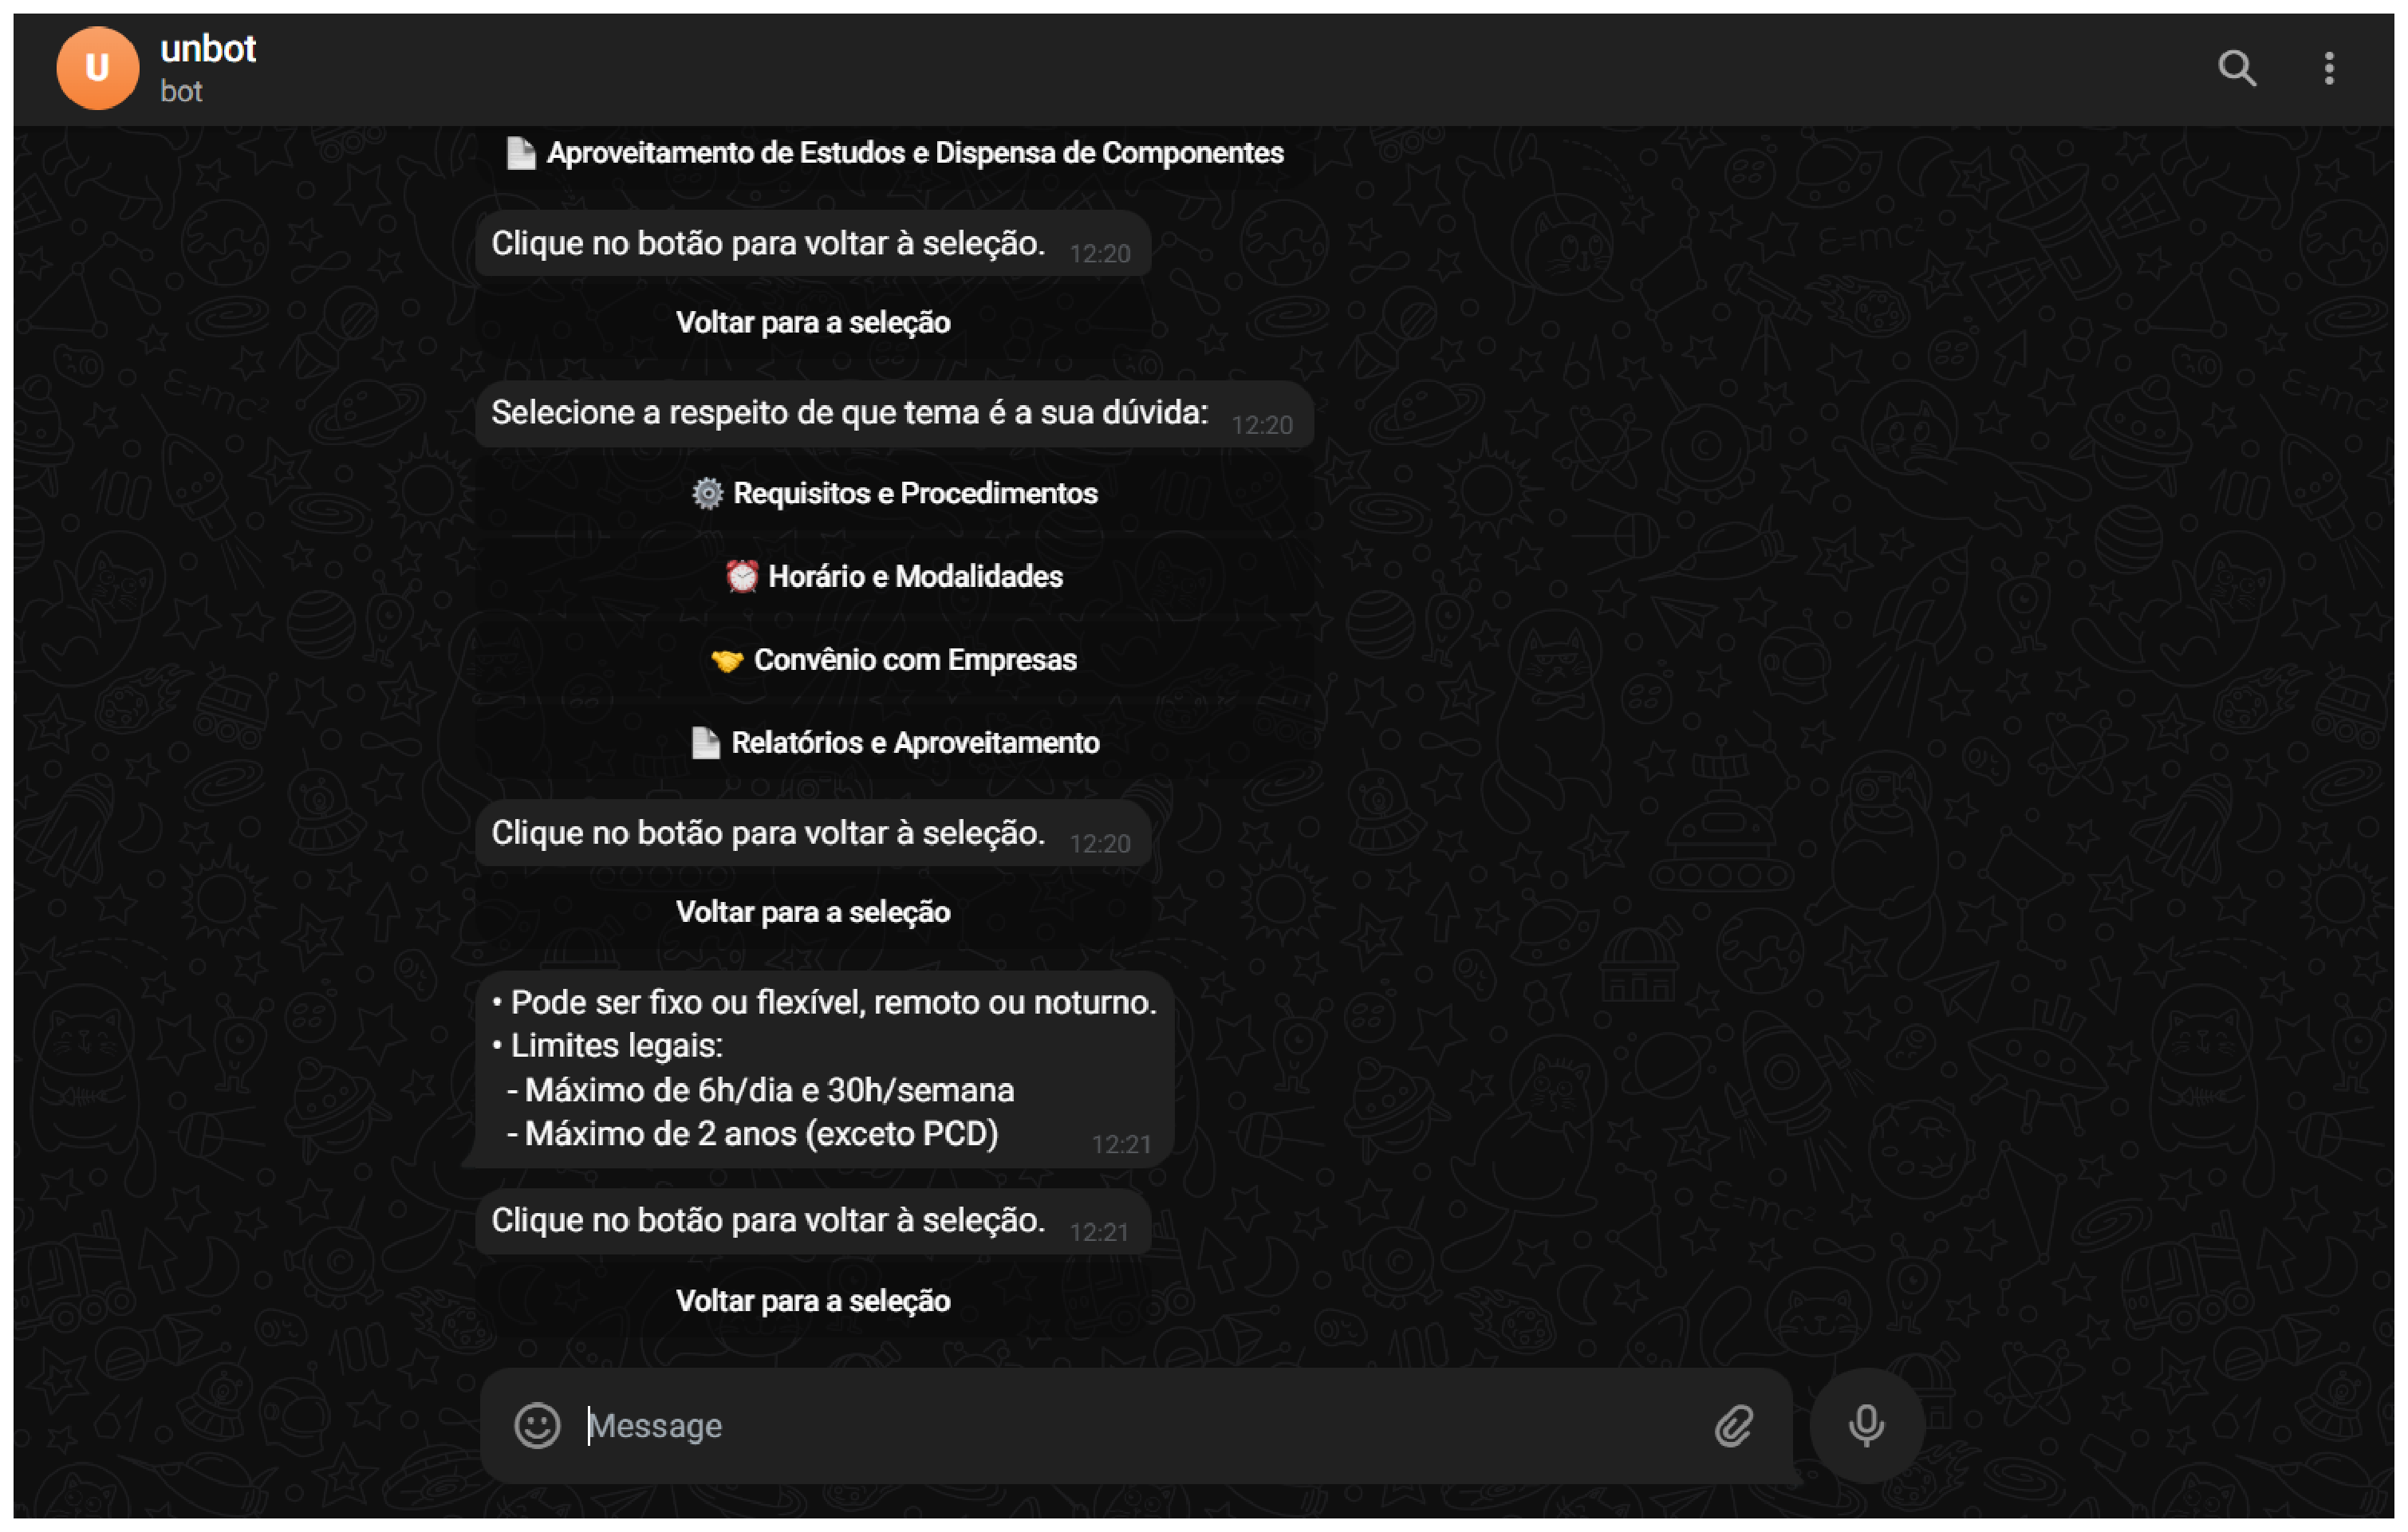
\includegraphics[width=1\linewidth]{./figuras/tela bot opcoes.eps}
	\caption{Tela de opções}
	\footnotesize Fonte: Autores.
	\label{fig06}
\end{figure}

